\smallframetitle

\section{Semaine du 21/05/24 au 28/05/24}
\insertsectionframe

\subsection{Statistiques stations de bases - départements}
\insertsubsectionframe

\begin{frame}{Méthodologie}
    On va utiliser une base de donnée complémentaire, reprise de celle trouvée l'année dernière.

    \begin{block}{Une nouvelle base de donnée\footnotemark}
        Cette base de donnée renseigne, par département, la \textbf{superficie} (en $\unit{km^2}$), la \textbf{population} et la \textbf{densité de population} au $\unit{km^2}$.
    \end{block}
    
    A partir de cette base, on va donc pouvoir extraire le nombre d'habitants par stations (normalisé par la taille du département) et la densité de station par département.

    \begin{block}{Calcul du nombre d'habitants par stations}
        Soit $\lambda$ le nombre que l'on cherche. Tout d'abord, on se donne $\gamma$, le rapport entre le nombre d'habitant et la surface du département, qui est donné par la densité de population.
        Ensuite, on calcule notre résultat comme suit :$$\lambda = \text{nombre de stations du département}\div\gamma$$
    \end{block}

    \footnotetext{\url{https://france.ousuisje.com/departements/classement/superficie.php}}
\end{frame}

\begin{frame}{Nombre d'habitants par stations}
    \begin{figure}
        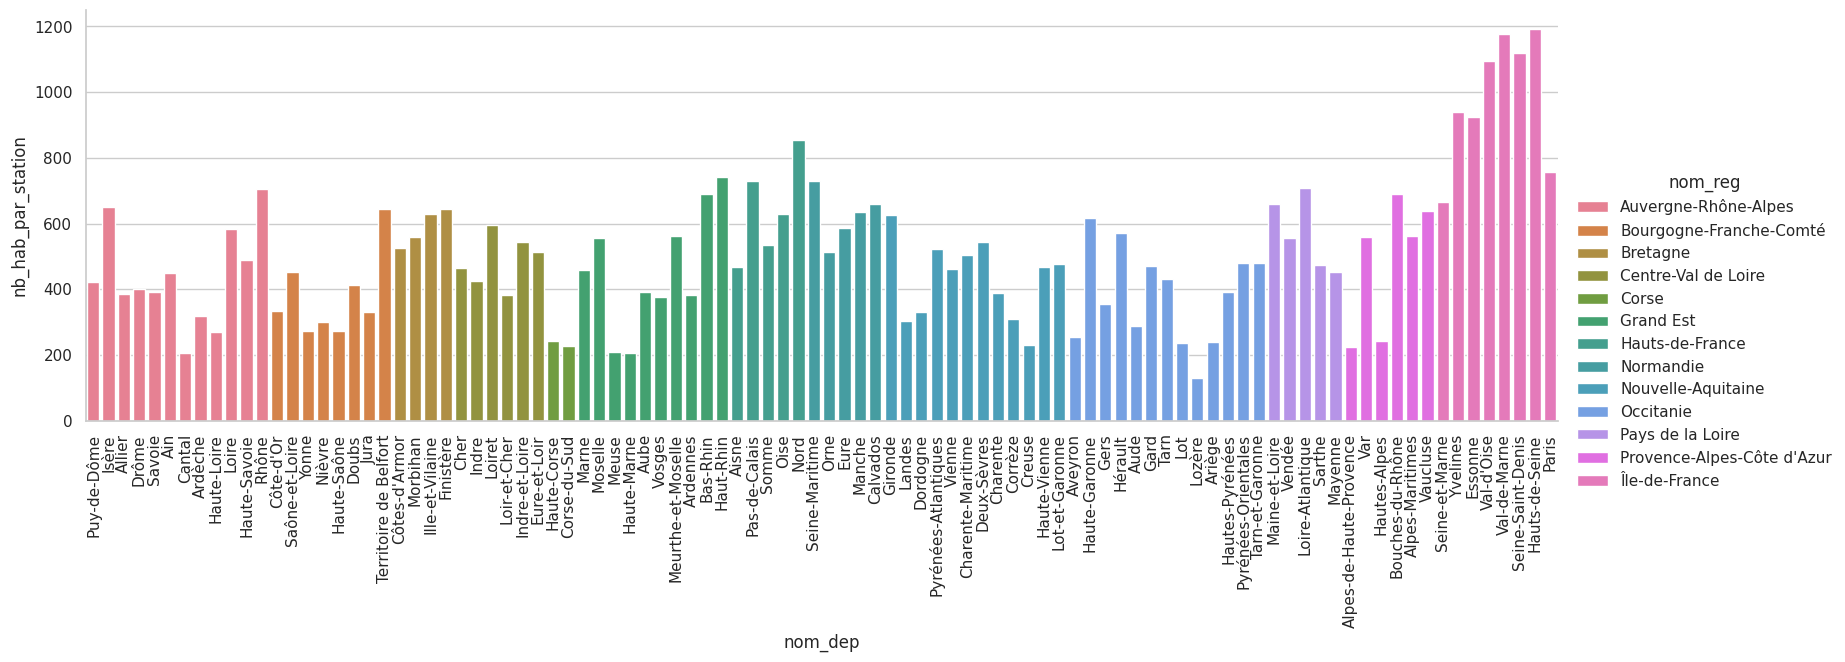
\includegraphics[width=0.9\paperwidth]{images/barplots/nb_hab_par_station_par_dep.png}
        \caption{\label{fig:nb_hap_par_stat_par_dep}Répartition du nombre d'habitants par station, en fonction du département}
    \end{figure}
\end{frame}

\begin{frame}{Densité de stations (1/2)}
    \begin{figure}
        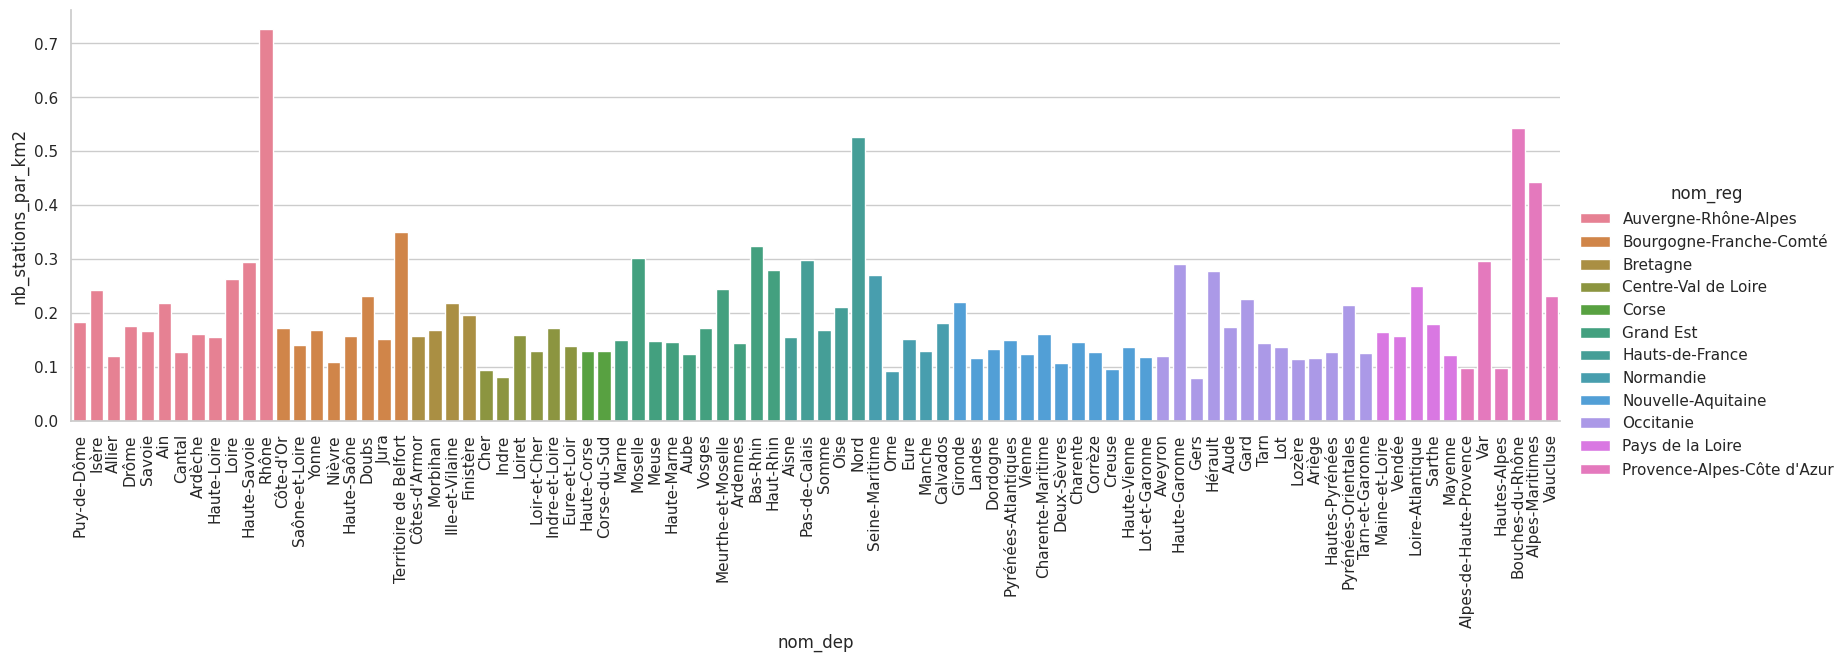
\includegraphics[width=0.9\paperwidth]{images/barplots/densite_station_par_dep_sansIDF.png}
        \caption{\label{fig:densite_stat_ssIDF}Nombre de stations de base au $\unit{km^2}$, sans l'Île-de-France}
    \end{figure}
\end{frame}

\begin{frame}{Densité de stations (2/2)}
    \begin{figure}
        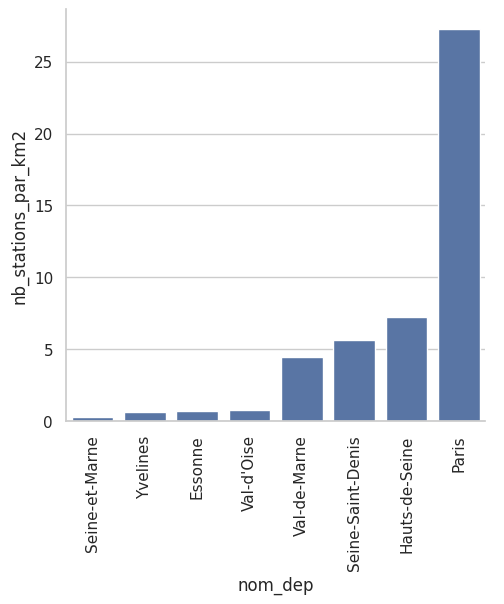
\includegraphics[height=0.55\paperheight]{images/barplots/densite_station_par_dep_IDF.png}
        \caption{\label{fig:densite_stat_IDF}Nombre de stations de base au $\unit{km^2}$, sur l'Île-de-France}
    \end{figure}
\end{frame}

\begin{frame}{Fréquences d'émission des stations 5G}
    \begin{figure}
        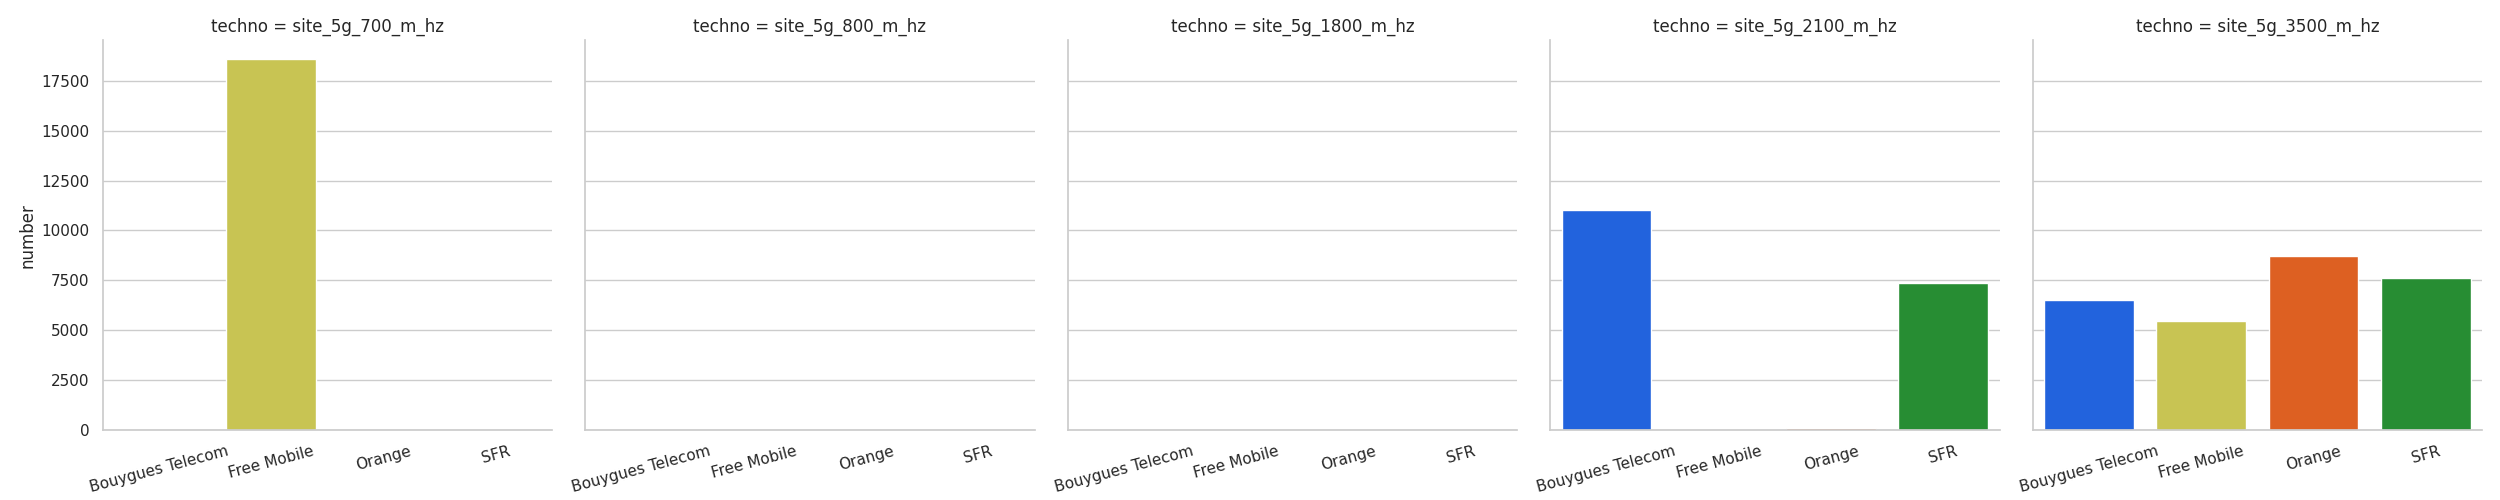
\includegraphics[width=0.9\paperwidth]{images/barplots/5G_freq.png}
        \caption{\label{fig:5g_freq}Répartition des fréquences d'émission des stations 5G, en fonction des opérateurs}
    \end{figure}
\end{frame}


\subsection{Détection automatique des villes}
\insertsubsectionframe

\begin{frame}{DBScan}
    \begin{block}{Principe}
        \begin{itemize}
            \item Méthode de référence de la classification à densité (détection de clusters en se basant sur la concentration de points);
            \item Se base sur deux paramètres : $\varepsilon$ et $n_{min}$ qui caractérisent respectivement la distance maximale pour que deux points soient considérés \og proches \fg{} et la quantité minimale de points proches pour qu'un cluster soit créé.
        \end{itemize}
    \end{block}

    \begin{block}{Inconvénients}
        \begin{itemize}
            \item Le choix du paramètre $\varepsilon$ est hasardeux;
            \item Ne se comporte pas bien avec des jeux de données avec des clusters de densité variable (certains clusters avec des points plus rapprochés que d'autres);
            \item Réagit mal au bruit;
            \item Est binaire : un point appartient ou n'appartient pas à un cluster, pas d'entre deux.
        \end{itemize}
    \end{block}
\end{frame}

\begin{frame}{Changement de métrique}
    Une façon d'améliorer le problème de mauvaise prise en compte du bruit est de changer de métrique :
    \begin{columns}
        \begin{column}{0.55\textwidth}
            \begin{block}{\emph{Core distance}}
                La \emph{core distance} d'un point du jeu de donnée est la distance entre ce point et son $k$-ième plus proche point ($k$ à fixer).
            \end{block}
        
            \begin{block}{Nouvelle métrique}
                La distance entre deux points $x$ et $y$ d'un jeu de donnée peut être définie comme la plus grande valeur entre les \emph{core distances} de $x$ et $y$ et la distance eucliedienne entre $x$ et $y$.
            \end{block}
        \end{column}
        \begin{column}{0.4\textwidth}
            \begin{figure}
                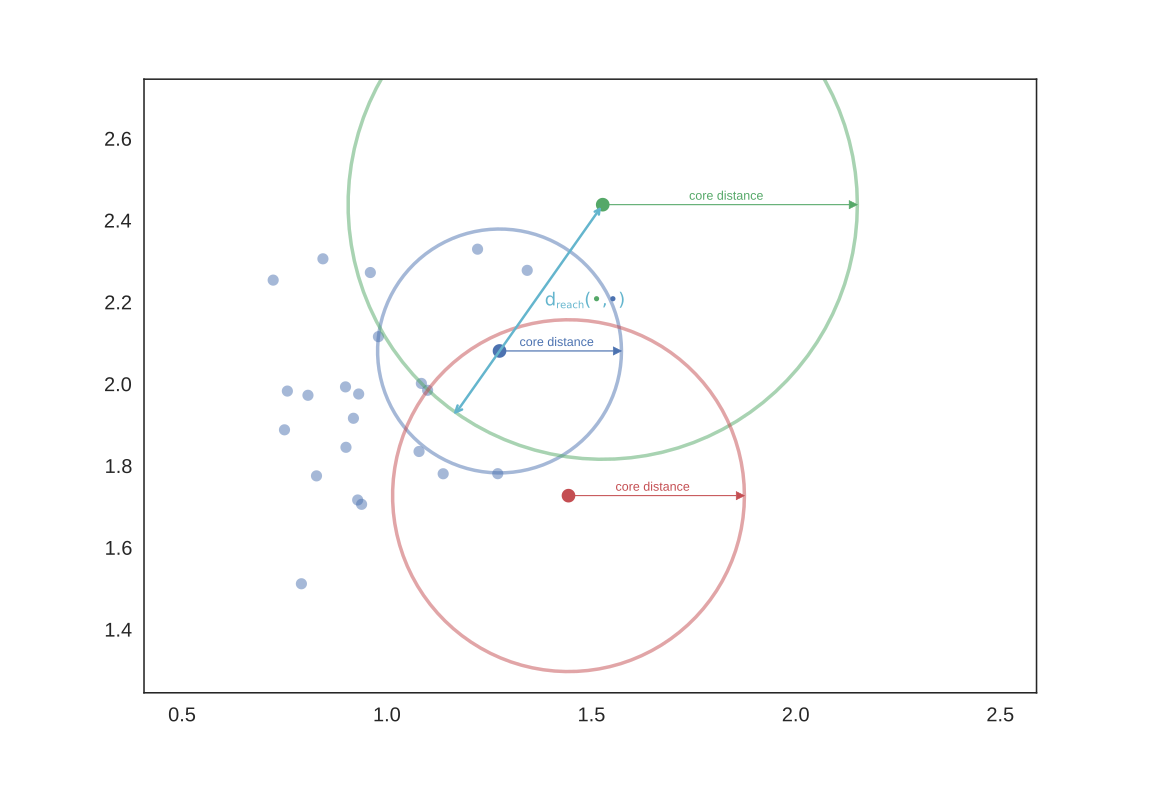
\includegraphics[width=0.6\paperheight]{images/metrique.png}
                \caption{\label{fig:metrique}Nouvelle métrique}
            \end{figure}
        \end{column}
    \end{columns}
\end{frame}

\begin{frame}{HDBScan (1/2)}
    \begin{block}{Principe général}
        Consiste à fusionner les méthodes de classification hierarchique adscendante et DBScan pour permettre de s'affranchir du paramètre $\varepsilon$.
    \end{block}

    \begin{block}{Étapes}
        \begin{itemize}
            \item Représenter les données par un graphe complet où chaque point est un sommet, puis valuer les arêtes par la métrique expliquée précédemment;
            \item Trouver un arbre couvrant de poids minimum dans ce graphe;
            \item Regarder quelles sont les composantes connexes du graphe en ne gardant que les arêtes dont le poids est inférieur à un certain seuil $\varepsilon$ que l'on augmente progressivement;
            \item On obtient alors un dendrogramme (on obient une partition pour chaque $\varepsilon$ fixé);
            \item On observe la persistance des classes de ce dendrogramme en fonction de la variation de $\varepsilon$.
        \end{itemize}
    \end{block}

\end{frame}

\begin{frame}{HDBScan (2/2)}
    \begin{block}{Avantages}
        \begin{itemize}
            \item Permet de prendre en compte les probèmes de classe à densité variable;
            \item En étudiant à quelle moment chaque point se retrouve exclu de sa classe au sein du dendrogramme, on obtient pour chaque point une probabilité d'appartenance à sa classe.
        \end{itemize}
    \end{block}

    \begin{block}{Application à notre cas d'utilisation}
        \begin{itemize}
            \item Appliqué de la même manière que DBScan : si un point est dans un cluster, alors on considère qu'il est en ville, sinon en campagne;
            \item La probabilité discutée précédemment permet de rajouter une incertitude sur l'appartenance (ou non) d'une station de base à une ville.
        \end{itemize}
    \end{block}
\end{frame}

\begin{frame}{Paramètres de sklearn.cluster.HDBSCAN}
    \begin{itemize}
        \item \texttt{min\_cluster\_size=5} : groupings smaller than this size will be left as noise;
        \item \texttt{min\_samples=None} : The number of samples in a neighborhood for a point to be considered as a core point;
        \item \texttt{cluster\_selection\_epsilon=0.0} : Clusters below this value will be merged;
        \item \texttt{max\_cluster\_size=None};
        \item \texttt{metric='euclidean'};
        \item \texttt{metric\_params=None};
        \item \texttt{alpha=1.0} : A distance scaling parameter;
        \item \texttt{algorithm='auto'} : Exactly which algorithm to use for computing core distances;
        \item \texttt{leaf\_size=40} : Leaf size for trees responsible for fast nearest neighbour queries when a KDTree or a BallTree are used as core-distance algorithms;
        \item \texttt{n\_jobs=None} : Number of jobs to run in parallel to calculate distances;
        \item \texttt{cluster\_selection\_method='eom'} : The method used to select clusters from the condensed tree;
        \item \texttt{allow\_single\_cluster=False} : allow the result to be a single cluster;
        \item \texttt{store\_centers=None};
        \item \texttt{copy=False}.
    \end{itemize}
\end{frame}

\begin{frame}{Résultats}
    \begin{figure}
        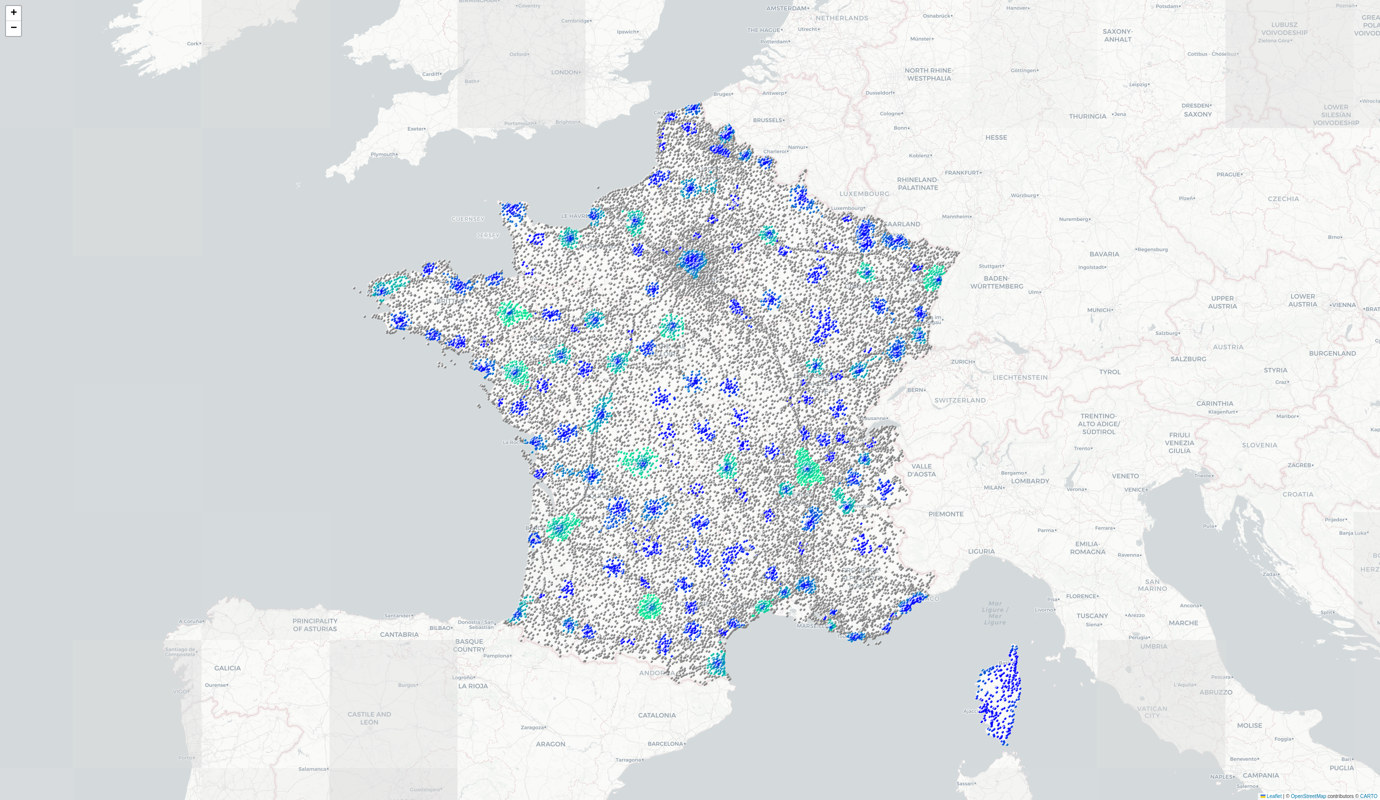
\includegraphics[width=0.9\paperheight]{images/villes_HDBSCAN.png}
        \caption{\label{fig:HDBSCAN}Application d'HDBScan \texttt{min\_cluster\_size=5}, \texttt{min\_samples=40}}
    \end{figure}
\end{frame}



